\documentclass[a4paper,12pt]{article}
\usepackage[utf8]{inputenc}
\usepackage[a4paper,margin=1in,footskip=0.25in]{geometry}

% science
\usepackage{amsmath}
\usepackage{array}
\usepackage{siunitx}
\usepackage{amssymb}

% code
% Default fixed font does not support bold face
\DeclareFixedFont{\ttb}{T1}{txtt}{bx}{n}{10} % for bold
\DeclareFixedFont{\ttm}{T1}{txtt}{m}{n}{10}  % for normal

% Custom colors
\usepackage{color}
\definecolor{deepblue}{rgb}{0,0,0.5}
\definecolor{deepred}{rgb}{0.6,0,0}
\definecolor{deepgreen}{rgb}{0,0.5,0}

\usepackage{listings}

% Python style for highlighting
\newcommand\pythonstyle{\lstset{
        language=Python,
        basicstyle=\ttm,
        morekeywords={self},              % Add keywords here
        keywordstyle=\ttb\color{deepblue},
        emph={MyClass,__init__},          % Custom highlighting
        emphstyle=\ttb\color{deepred},    % Custom highlighting style
        stringstyle=\color{deepgreen},
        frame=tb,                         % Any extra options here
        showstringspaces=false
}}

\newcommand\pythonstyleln{\lstset{
        language=Python,
        basicstyle=\ttm,
        morekeywords={self},              % Add keywords here
        keywordstyle=\ttb\color{deepblue},
        emph={MyClass,__init__},          % Custom highlighting
        emphstyle=\ttb\color{deepred},    % Custom highlighting style
        stringstyle=\color{deepgreen},
        frame=tb,                         % Any extra options here
        showstringspaces=false,
        numbers=left
}}

% Python environment
\lstnewenvironment{python}[1][]
{
    \pythonstyle
    \lstset{#1}
}
{}

\lstnewenvironment{pythonln}[1][]
{
    \pythonstyleln
    \lstset{#1}
}
{}

% Python for external files
\newcommand\pythonexternal[2][]{{
        \pythonstyle
        \lstinputlisting[#1]{#2}}}

% Python for inline
\newcommand\pythoninline[1]{{\pythonstyle\lstinline!#1!}}

% layout
\usepackage{float}
\usepackage{parskip}
\usepackage{graphicx}
\usepackage{longtable}
\usepackage{hyperref}
\usepackage[export]{adjustbox}
\usepackage{hhline}
\usepackage{chngcntr}

% referencing
\usepackage[style=apa]{biblatex}
\addbibresource{jump.bib}

% table centering
\renewcommand{\arraystretch}{1.3}
\newcolumntype{P}[1]{>{\raggedright\arraybackslash}p{#1}}
\newcommand{\tptt}{$\times\,$}

% figures labelings
\usepackage{chngcntr}
\counterwithin{figure}{section}

\usepackage{caption}
\usepackage{subcaption}
\usepackage{wrapfig}

% fancy page numbers
\usepackage{fancyhdr}
% bottom right
\pagestyle{fancy}
\fancyhf{}
\fancyfoot[R]{\thepage}
\fancypagestyle{plain}{%
    \renewcommand{\headrulewidth}{0pt}%
    \fancyhf{}%
    \fancyfoot[R]{\thepage}%
}
%go
\renewcommand{\headrulewidth}{0pt}

% extra maths commands
\usepackage{mathtools}
\DeclarePairedDelimiter\ceil{\lceil}{\rceil}
\DeclarePairedDelimiter\floor{\lfloor}{\rfloor}

\newcommand{\tvec}[1]{\boldsymbol{#1}}
\newcommand{\tunit}[1]{\boldsymbol{\hat{#1}}}
\newcommand{\tmag}[1]{\|#1\|}
\newcommand{\tang}[1]{\left\langle #1 \right\rangle}
\newcommand{\ta}{\tvec{a}}
\newcommand{\tv}{\tvec{v}}
\newcommand{\tp}{\tvec{p}}
\newcommand{\tpar}[2]{\begin{bmatrix}#1\\#2 \end{bmatrix}}
\newcommand{\tpars}[3]{\begin{bmatrix} #1\\#2\\#3 \end{bmatrix}}
\newcommand{\tfx}{\mathcal{X}}
\newcommand{\tfy}{\mathcal{Y}}

\newcommand{\I}{{i\mkern1mu}}

\linespread{1.5}

\usepackage{hyperref}

\title{The Optimization of Air Movements within a Video Game Jump Action}

\author{Word Count: $<$ 4000}
\date{}

%\includeonly{
    %sections/jumping.tex,
 %   sections/models.tex
%}
\begin{document}

    \maketitle

    \newpage
    % texcount

    \newpage

    \tableofcontents

    \newpage


% introduction
%  research question
%  reasons
%  definitions

% mechanics
%  vectors and quirk dot product
%  complex numbers and differential equation

% Z-axis modelling
%  continous updating
%  discrete updating
%  evaluation

% XY-axis modelling
%  continous straightline
%  continous right turning at fixed rate
%  continous euler-lagrange
%  discrete velocity maximizing
%  discrete velocity maximizing with let go
%  discrete displacement maximizing
%  result, significance

% Conclusion


% first model and my best attempt



\section{Introduction}

%\paragraph{Research Question:}

In this essay, I will be optimizing the jumping displacement in the video game ``Counter Strike, Source''. This is a competitive game that I enjoy where you control a ``player'' in a simulated 3D space doing objectives. While normally the player's movement --- the velocity in particular --- in the game is limited by a value for fairness sake, I realized that it can be exceeded under certain circumstances. This is extremely helpful in a game where your movement determines you and your team's success, therefore, I sought to master this technique with mathematics.

% This is a result of a friend sending me inhuman like videos of people playing the game, ``exploiting'' it to make themselves move much faster in midair than intended. Out of interest, I found this exploit online and wanted was hooked --- but it is difficult to utilize a new piece of knowledge without understanding it. I want to perfect this act of incredible movement optimally.

To achieve this I would need to select and concentrate on a single matrix to evaluate my models against, because of the myriad uses of this technique in game; I chose the displacement traveled in a player jump for its simplicity. My research question was therefore:
\begin{quote}
    To what extent can a player travel in displacement through a jump action on an even plane within the video game ``Counter Strike, Source''?
\end{quote}

% definition
\subsection{Mathematical definition}
The question is easier to analyze when defined mathematically, but in order to explain the mechanics, let's first consider an analogy to real life. Consider the modeling of a student's location within a school: we designate him with a position, velocity, and acceleration, then by simply applying the classical laws of motion we can accurately locate him at all times. In the context of the video game, the student is the player, the school is a ``map'', and a similar ``law of motion'' is applied programmatically. Additionally, the game uses ``hammer units'' as units of space and seconds as units of time in its virtual environment.


From my personal experience with the game, and from external sources on this topic \parencite{Kered13}, The player's position are coordinates of three real numbers, representing its 3D displacement against the origin coordinate $\tang{0,0,0}$. I will denote its position by a bold $\tp$ using vector notation
\[
    \tp = \tang{x, y, z} \quad \text{where} \, x, y, z \in  \mathbb{R}.
\]

\begin{wrapfigure}{r}{0.40\textwidth}
    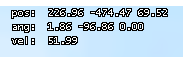
\includegraphics[width=0.37\textwidth,right]{assets/1coords.png}
    \caption{Player Coordinates}
    \label{fig:1coords}
\end{wrapfigure}

The game stores the velocity of the player as a real 3-vector as well, which I will denote by a bold $\tv$. The magnitude of these positions, velocities, and any real 3-vectors are computed using Pythagoras's theorem: here is the equation for the player's speed,
\[
    \tmag{\tv} = \sqrt{\tv_x^2+\tv_y^2+\tv_z^2}.
\]


Figure \ref{fig:1coords} is a snapshot of the game showing the two value; the player is at position $\tang{226.96, -474.47, 69.52}$ with a velocity of magnitude $51.99$ (the displayed values are rounded to 2 p).


The game also keeps track of the time elapsed, and updates the player's position and velocity $n$ times a second, called $n$ ticks. This value is often $64$, meaning $64$ evenly spaced updates in a second. I will represent the time between updates as $\tau$, a value of
\[
    \tau = \frac{1}{64} = 0.015625 \si{s}.
\]

\begin{wrapfigure}{r}{0.40\textwidth}
    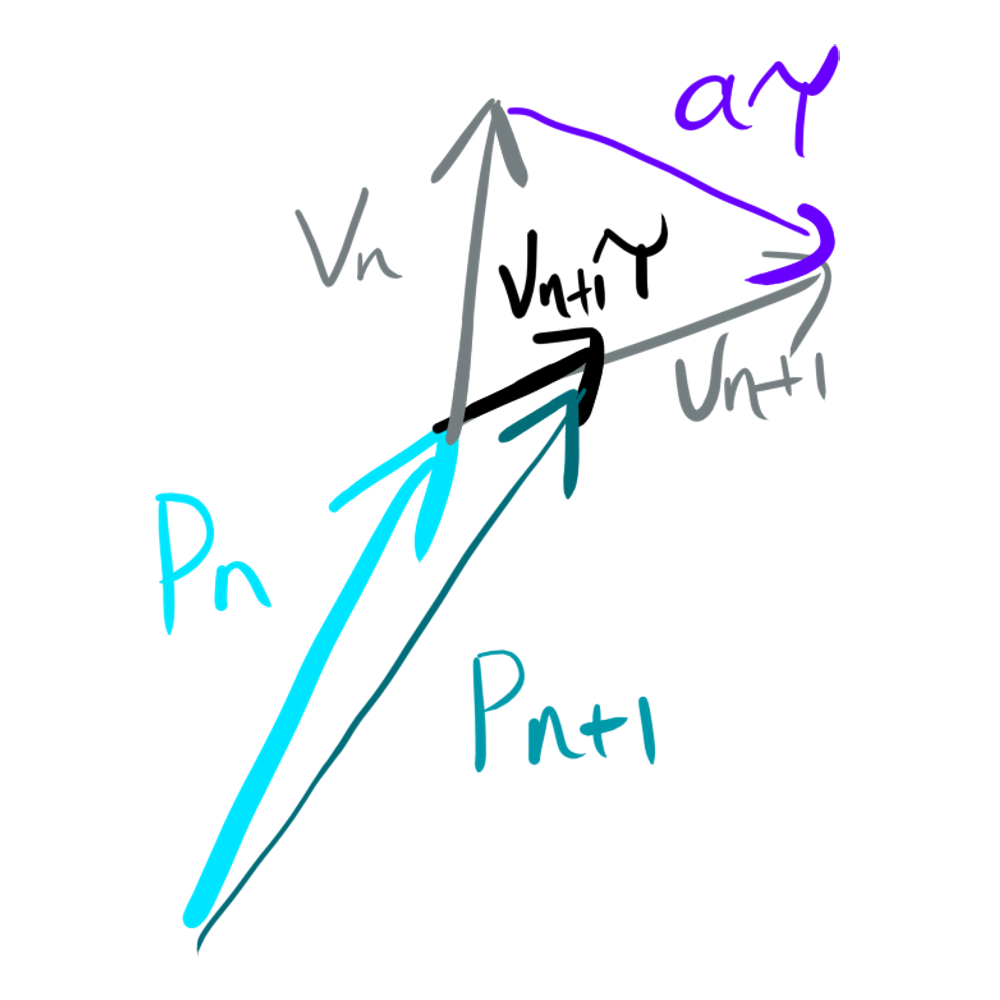
\includegraphics[width=0.37\textwidth,right]{assets/1vecadd.png}
    \caption{Every frame}
    \label{fig:1vecadd}
\end{wrapfigure}

Moreover, the acceleration $\ta$ is also a real 3-vector. It is computed every update from the ``wishing'' direction $\td$ --- another real 3-vector --- of the player, which is then applied onto the velocity $\tv_n$ using Euler's method. The position $\tp_n$ is then updated with the new velocity $\tv{n+1}$ through the same method. This sequential process can be represented by the difference equations
\begin{align}
    \tv_{n+1} &= \tv_n + \ta \tau\\
    \tp_{n+1} &= \tp_n + \tv_{n+1} \tau.
\end{align}

The process of one such update is called a ``frame'', and can be visualized through vectors scalings and additions as figure \ref{fig:1vecadd} demonstrates.

It is therefore obvious to see that the player position and velocity are discrete functions of time. While it may be conventional to represent the time parameter as subscripts, I decided against it and to write it with a continuous function syntax. This is because the powerful optimization techniques such as calculus only apply to continuous functions, and I conjecture that the small delta time $\tau$ justifies such transition from discrete to continuous. Beneficially, the function syntax allows for such continuous position and velocity, while still retaining the faithful discrete time properties in case I wish to fall back upon it. To summarize, I decided to model the motion of the player with the functions $\tp(t)$ and $\tv(t)$, where $t$ is time elapsed in seconds from the start of the jump, with the updating process now approximated by differential equations:
\begin{align}
    \tv'(t) &= \ta(t) \label{eq:1de1}\\
    \tp'(t) &= \tv(t) \label{eq:1de2}.
\end{align}

Ultimately, the problem can be formally state as so:
\begin{quote}
    Given initial position $\tvec{p}(0)$ and velocity $\tvec{v}(0)$ as three dimensional vectors when the player initializes a jump event. If $\ta(t)$ is the acceleration vector function representing the player acceleration at every time $t$, with $\tv(t)$ and $\tp(t)$ being the respective derived velocity and position of the player at time $t$, what is the maximum displacement $\tmag{\tp(t_f) - \tp(0)}$ achievable if $t_f$ is the total time of the jump?
\end{quote}
%The problem originated from my personal curiosity within the limitations of the video game ``Counter Strike'' that occupies a large part of my life. It came about as I was getting into the community of counter-strike long jumping --- a community aiming to exploit the video game's physics to achieve the longest jumping distance. Therefore I want to explore this optimization problem with various methods in an extended essay to further improve my knowledge within this ``niche`` community.

%\subsection{Defining the problem}
%The ``source'' game engine (citation) is the engine of plenty of popular videos games in terms of handling the players, their surroundings, and their respective physical interactions. It allows freedom in setting various engine constants that fit each video game's playstyle --- with the constants of ``Counter Strike - Source`` being used as a reference throughout this exploration. I will attempt to define the problem mathematically in this section.

% from p0 to p1, and to finishing this essay
%Firstly, here is a run down of all the notations used in this analysis:
%
%All n-dimensional vectors are represented in bold styles like
%\[
%    \tvec{v},
%\]
%their magnitudes, or length are denoted by two double vertical lines, with the components of a vector written as a subscript $x$, $y$, or $z$ like
%\[
%\tmag{\tvec{v}} = \sqrt{v_x^2 + v_y^2 + v_z^2}.
%\]
%
%The vector can also be expanded into its components, and is written with angled brackets or with square brackets:
%\[
%\tvec{v} = \tang{v_x, v_y, v_z} = \tpars{v_x}{v_y}{v_z}.
%\]
%
%The unit vectors are vectors scaled down by their magnitudes, resulting in a magnitude of 1, and is written with a hat on top:
%\[
%\tunit{v} = \frac{\tvec{v}}{\tmag{v}}.
%\]
%
%The dot product between two vectors $\tvec{v}$ and $\tvec{w}$ is defined by
%\[
%\tvec{v} \cdot \tvec{w} = v_x w_x + v_y w_y + v_z w_z + \ldots.
%\]
%
%In addition, the absolute, floor, and ceiling piecewise functions are represented with
%\[
%    |x|, \floor*{x}, \ceil*{x}.
%\]
%
%Due to the nature of the source engine, the problem may be represented and optimized differently because of the use of discrete time frames rather than continuous time. But experimentally the differences are small and insignificant --- this will be shown later. Both approaches will thus be used, sometimes interchangeably.
%

%
%\subsection{Source mechanics}
%\label{sec:source}
%While the problem may look simple in the context of kinematics and projectile motions, the ``quirks'' in the source engine will increase its complexity. Therefore it is necessary to explore the specifics of the physics engine.
%
%The engine time unit is in seconds; the engine distance unit is in hammerunits (hu), which are to be implied for the rest of the analysis. The player's position and velocities are represented by 3-vectors $\tp$ and $\tv$ in the engine, which are updated every frame by the player controllable acceleration 2-vector $\ta$. Commonly, the source engine runs at an integer number of frames per second (citation), the number $64$ will be used from now. Let $\tau$ be the time between frames (also know as $\Delta t$) and it has a value of $\tau = \frac{1}{64} \approx 0.0156 \si{s}$. For every $\tau$ seconds after $t=0$, the velocity is updated in the following sequence (citations):
%\begin{enumerate}
%    \item Apply gravitational acceleration
%    \item Apply friction onto velocity
%    \item Calculate magnitude of movement acceleration
%    \item Apply movement acceleration
%\end{enumerate}
%
%% took 45 frames, v0 = 284hu/s, 60fps
%\paragraph{Step 1} Let $g$ be the gravitational acceleration on the $z$ axis, it is set by an engine constant \verb|sv_gravity| (citations) --- represented by variable $-g$ set to $800$ within the game in question. Using a method called leapfrog interpolation, and let $\tv'$, $\tp'$ be the new velocity, position next frame, the operation is (assuming $g$ is negative)
%\begin{align}
%    \tv'_z &= \tv_z + g\tau \label{eq:gv}\\
%    \tp'_z &= \tp_z + \tv_z\tau + \frac{1}{2}g\tau^2 \label{eq:gp}.
%\end{align}
%
%Because the updates reflect the kinematic equations of a projectile with constant acceleration, it can be treated with assumption of continuous time and will be evaluated separately against the $x$ and $y$ motions.
%
%
%\paragraph{Step 2} Let $\lambda(\tv)$ be the friction function. For the player is in the air, no friction will be applied and we can set $\lambda(\tv) = \tv$. After this section, the $\lambda$ function will be omitted as we are only considering air motions.
%
%\paragraph{Step 3} The source engine limits the player velocity through an engine constant \verb|sv_maxspeed| ($L$) set to $30$ in air. However, the speed is limited by the projection of the velocity vector $\tv$ onto the acceleration vector $\ta$, with the player having control of $\ta$ at all times (figure \ref{fig:speedlimit}).
%
%\begin{wrapfigure}{r}{0.40\textwidth}
%    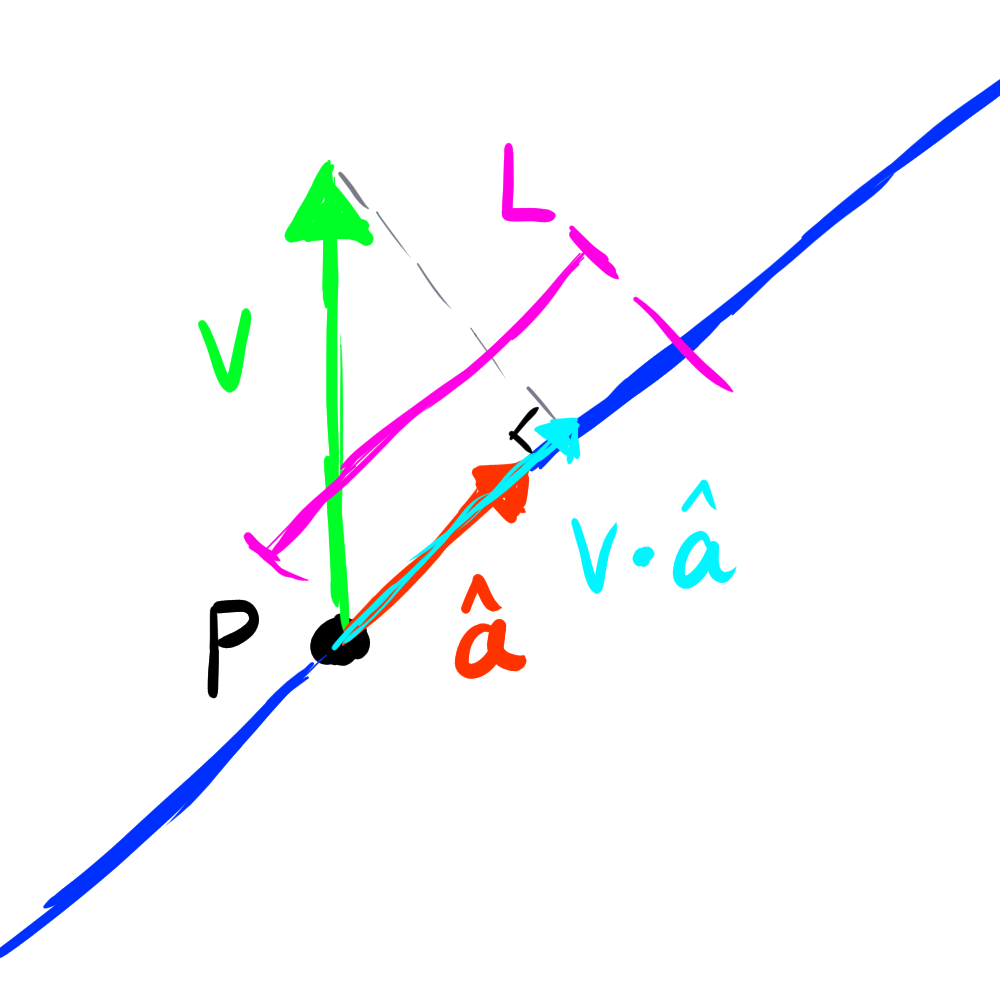
\includegraphics[width=0.37\textwidth,right]{assets/speedlimit.png}
%    \caption{The speed limit}
%    \label{fig:speedlimit}
%\end{wrapfigure}
%
%Let $w$ be the magnitude of the applicable acceleration this frame. It can be defined as a piecewise function as
%\[
%w = \begin{cases}
%    \gamma_1 & \gamma_2 \ge \gamma_1\\
%    \gamma_2 & \gamma_1 > \gamma_2 > 0\\
%    0 & 0 \ge \gamma_2,
%\end{cases}
%\]
%where the definition of $\gamma_1$ and $\gamma_2$ are:
%\begin{align*}
%    \gamma_1 &= LA\tau\\
%    \gamma_2 &= L - \tv \cdot \tunit{\ta},
%\end{align*}
%where the dot product $\tv \cdot \tunit{\ta}$ with the unit acceleration vector represents the projection of velocity onto the acceleration vector.
%
%The variable $\gamma_1$ is a constant represents the highest acceleration and is proportional to the engine constant \verb|sv_airacclerate| ($A$), and \verb|sv_maxspeed| ($L$); variable $\gamma_2$ is a function of $\tv$ representing the signed the difference between $L$ and the projected velocity.
%
%When $\gamma_2$ is negative, meaning the projected velocity is larger than the max speed, no acceleration will occur and $w=0$; when $\gamma_2$ is positive but below $\gamma_1$, meaning that adding the full acceleration will overshoot the max speed, only the difference between the max speed and the current projected velocity is applied, bringing the player to the speed limit on the next frame and $w=\gamma_2$; when $\gamma_2$ is larger than $\gamma_1$, only the upper-bound acceleration is applied and $w=\gamma_1$.
%
%
%
%\paragraph{Step 4} The new velocity on the next frame $\tv'$ (note that we assume step 1 has already been applied this frame) is the combination between the friction and movement acceleration:
%\begin{align}
%    \tv' &= \lambda(\tv) + w \tunit{\ta}\label{eq:dis_vel},
%\end{align}
%with the position being updated without interpolation ($\tp'$):
%\[
%\tp' = \tp + \tv' \tau.
%\]
%
%% jumping mechanics
%% took 45 frames, v0 = 284hu/s, 60fps
%Additionally, the mechanics of initiating a jump action can also be modelled mathematically. By recording myself jumping ingame at 60 frames per second (picture), I've obtained that a jump is represented by an impulse applied on the player, setting its z-axis velocity $v_{0z}$ to around $+280\pm10$ the frame after jumping. The player then takes around $45 \pm1$ video frames to land, meaning an airtime of $45 / 60 =0.75\pm 0.02\si{s}$. Therefore the initial velocity is restricted by $\tv_z = 280\pm10$.
%
%% summarize
%To summarize, every $\tau$ seconds after $t=0$ the velocity is updated by gravity in the z-axis, and by the player's movement acceleration in the x,y-axis. The latter is limited so that the projection of the new velocity never exceeds the engine constant \verb|sv_maxspeed| of 30 in air. Therefore for some time $t$, the velocity next frame $\tv(t+\tau)$ is
%\begin{align*}
%    \tv(t+\tau) &= \tang{\tv_x(t) + w \tunit{a}_x, \tv_y(t) + w\tunit{a}_y,\tv_z(t) + g\tau}\\
%    \tp(t+\tau) &= \tang{\tp_x(t) + \tv(t+\tau)_x \tau, \tp_y(t) + \tv(t+\tau)_y \tau, \tp_z(t) + \tv_z(t)\tau + \frac{1}{2}g\tau^2}.
%\end{align*}


\section{Basic Models}
I want to set some baseline movement models in this section, for it not only helps me to visualize the problem, but can also test my conjuncture in the negligibility of the continuous approximations.

My approach to maximize player jumping displacement can be described in sections. Firstly, I wish to find an optimal starting condition, then an analogy can made with projectile motion, leading to the precalculation of the vertical motion; Secondly, I hope to model the mechanics between the remaining two axis of motion; Lastly, I will fit various acceleration models base on my intuition, calculus, and even the switching to polar coordinates.

% straight line
\subsection{Key idea and boundary condition}
The key idea that will be repeated throughout this analysis is the extend that maximizing the player velocity will maximize the displacement. I hypothesized this from the position differential equations in Eq. \ref{eq:1de2}, that under the assumption of constant velocity, the final displacement will be proportional to that constant:
\begin{align*}
    \tp'(t) &= \tv(t)\\
    \tp(t) &= \int \tv(t) \, dt\\
    &= t(\tv(t)) + \tp(0) = t(\tv(t)) + \tvec{0},\\
    \tp &\propto \tv(t).
\end{align*}

Therefore, I was able to set an optimal initial velocity for the player, also known as the boundary condition of the problem. For we are maximizing the jump displacement, and higher velocity equates to higher displacement, it is reasonable to set the initial velocity as high as possible. So
\[
    \tmag{\tv} = 250,
\]
where $250$ is the player's fastest ground running speed.


\begin{figure}[H]
    \centering
    \begin{minipage}{.5\textwidth}
        \centering
        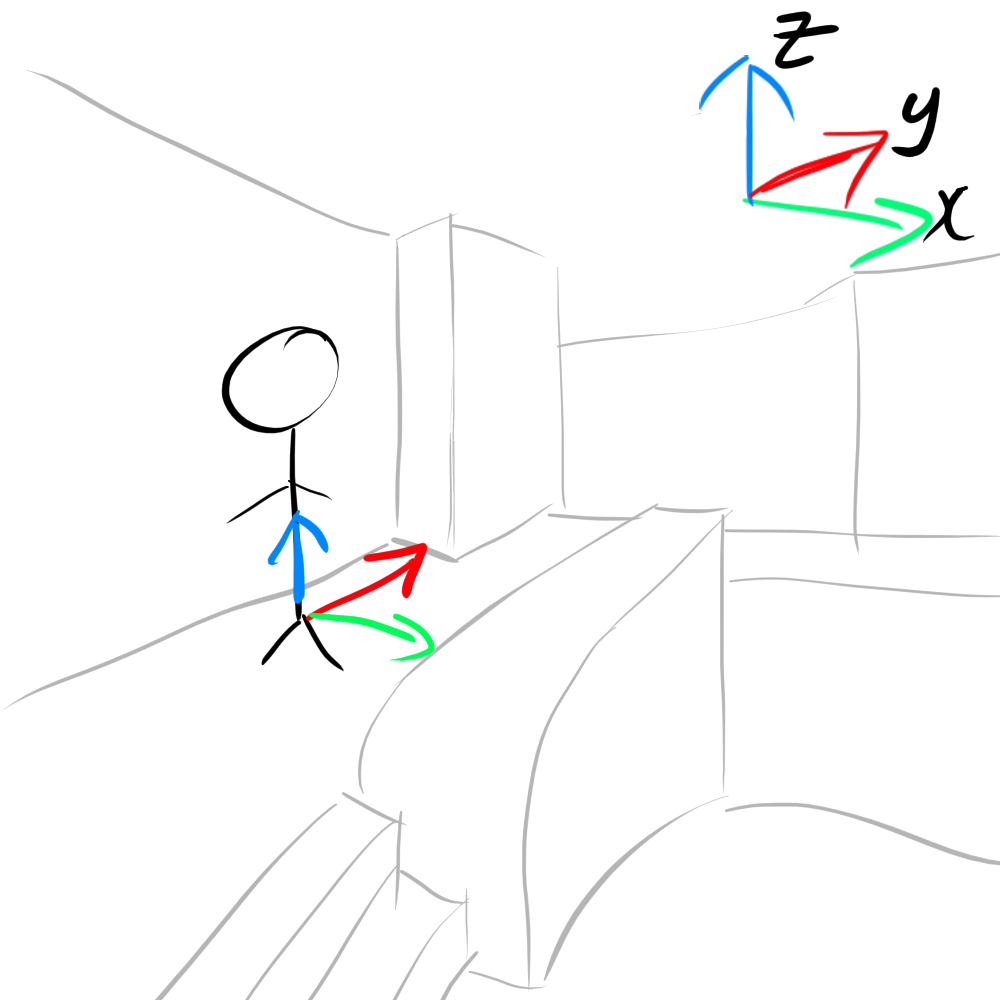
\includegraphics[width=0.9\linewidth]{assets/1coordinates.png}
        \caption{The coordinate system}
        \label{fig:1coordinates}
    \end{minipage}%
    \begin{minipage}{.5\textwidth}
        \centering
        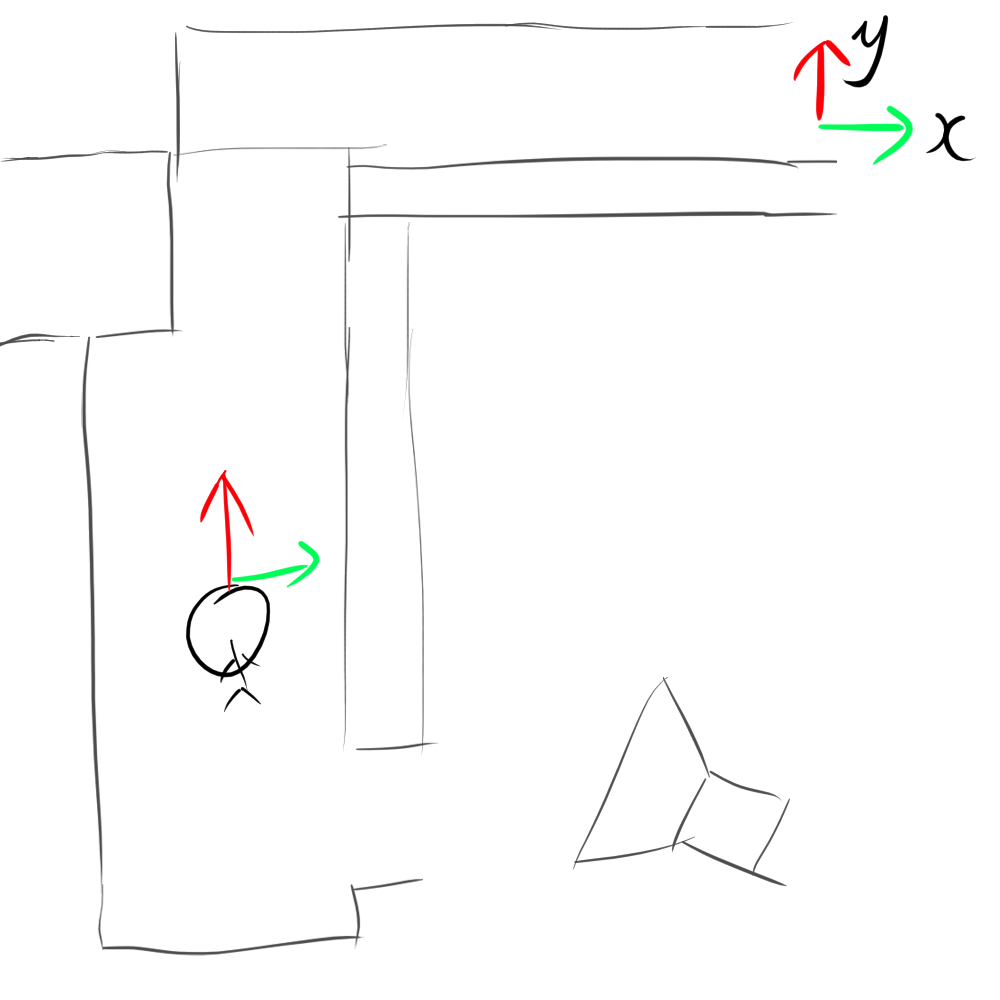
\includegraphics[width=0.9\linewidth]{assets/2coordinate_topdown.png}
        \caption{The top down view}
        \label{fig:2coordinates_topdown}
    \end{minipage}
\end{figure}

\begin{wrapfigure}{r}{0.40\textwidth}
    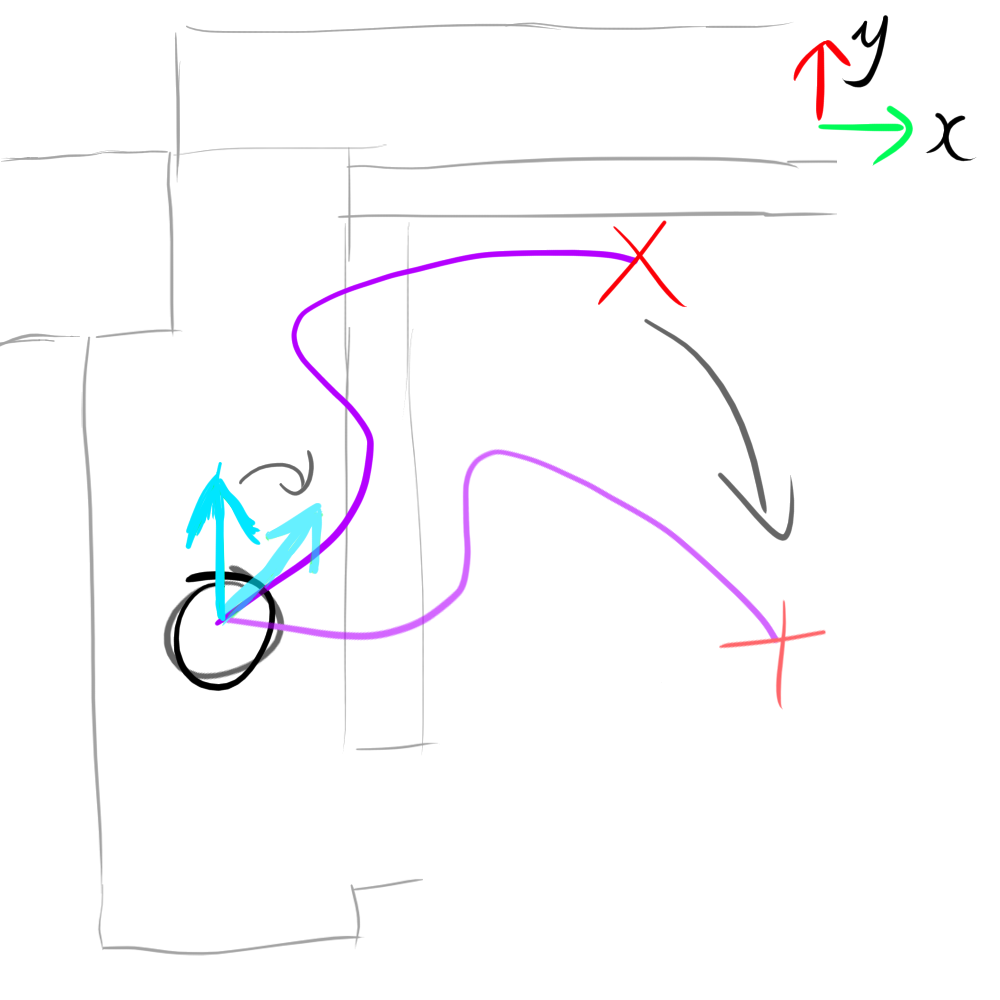
\includegraphics[width=0.37\textwidth,right]{assets/2turning.png}
    \caption{Rotational Invariant (the player wishes to go rightwards)}
    \label{fig:2turning}
\end{wrapfigure}

Furthermore, it should be noted that the problem is rotationally invariant when viewed top down. Let the z-axis denote the vertical height of the player, and the x,y-axis to be the plane displacement from a top down view (see figure \ref{fig:1coordinates}, figure \ref{fig:2coordinates_topdown}). By considering only the x,y-axis --- and the z-axis remaining constant before and after the jump --- I realized that an optimal strategy does not depend on the angle of the initial velocity vector within the plane, for unless we somehow ended up behind our initial direction, it is always possible to rotate the initial velocity such that we travel in a desired direction of displacement (see figure \ref{fig:2turning}). This meant that the optimal initial velocity is not restricted to a certain direction, but for the sake of consistency between models, I shall use the initial velocity pointing in the y-axis:
\[
    \tv = \tang{0, 250, 0}.
\]

\subsection{Straight Line}
With the key idea and boundary condition in mind, I attempted a straight line model. This model has the player accelerate and move in a straight line, for mathematics has taught me that the shortest distance between two points comes from a line, resulting in less time needed to travel a long distance, which is helpful in optimizing displacement over time. To achieve this, the player would need to accelerate along the y-axis, for that is in the direction of its initial velocity, which maximizes speed at all times, and would theoretically result in the largest displacement. Realistically, this will be equivalent to pressing down ``w'' and not moving the mouse.
% do model!!

\begin{wrapfigure}{r}{0.40\textwidth}
    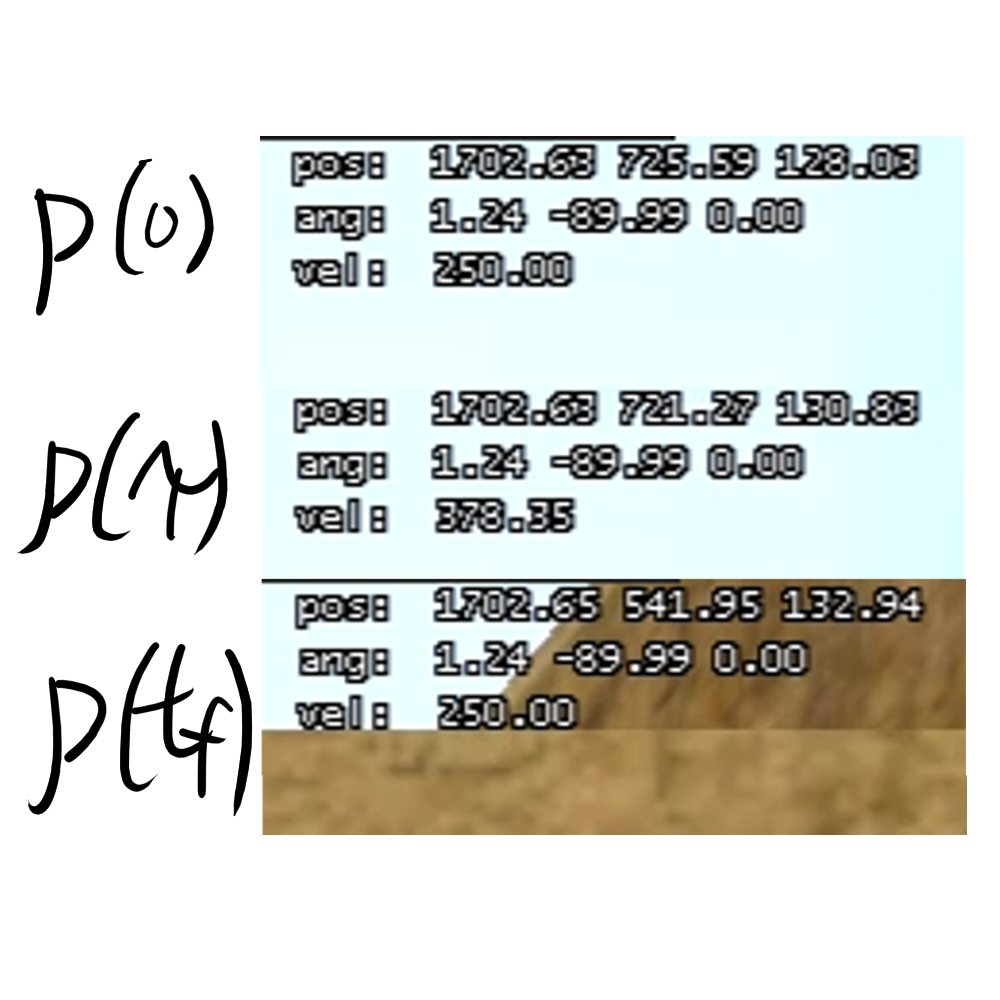
\includegraphics[width=0.37\textwidth,right]{assets/2straightjumping.png}
    \caption{Straight Jumping}
    \label{fig:2straightjumping}
\end{wrapfigure}

To test this model, I recorded myself jumping and doing the actions described above. Figure \ref{fig:2straightjumping} shows the coordinates of the player at the start of the jump $\tp(0)$, the first discrete time of the jump $\tp(\tau)$, and the end of the jump $\tp(t_f)$, where $t_f$ denotes the duration of the jump. % explain




%% 44 frames
% discuss vertical axis

% evantually my best, and as a model

% try it

% TODO: do the euler-lagrange only with max speed!!

%\section{Vertical motion}
Universal across the various metrics are the vertical motion of the player. Firstly notice that the z-axis motion is separated from the x,y-axis motion, meaning that it can be computed on its own.

Let $p$, $v$, $a$ be the z-axis position, velocity, and acceleration as a function of time $t$ and engine constants $S$, also define $p_0$, $v_0$ to be the initial conditions. Because of the velocity update in equation \ref{eq:gv}:
\[
\frac{\Delta v}{\tau} = g,
\]
because $\tau$ is very small, it can be assumed that:
\[
v' = g.
\]
Similarly, the position update can also be assumed to be continuous (equation \ref{eq:gp}):
\begin{align*}
    \frac{\Delta p}{\tau} &= v(t+\tau)\\
    p' &= v.
\end{align*}
Therefore it is possible to compute the airtime of the player upon a jump action. For the acceleration of gravity is constant, the kinematic equations may be used (citation).
\begin{align*}
    s &= s_0 + ut + \frac{1}{2} a t^2\\
    0 &= 0 + v_0 t + \frac{1}{2} g t^2\\
    \text{therefore:}&\\
    t &= \frac{-v_0 \pm \sqrt{v_0^2}}{g}\\
    &= \frac{-2v_0}{g} \,\, \text{or} \,\, 0.
\end{align*}
Because $t=0$ is the first frame when the player executes the jump action, the airtime is the first root of the quadratic, and therefore:
\begin{align*}
    t &= -2 \frac{v_0}{g}\\
    &= -2 \times \frac{280\pm 10}{-800}\\
    &= 0.70 \pm 0.03 \si{s}
\end{align*}

The result is very similar to the recorded airtime of $0.75\pm 0.02$ with their uncertainty overlapping, the assumption of a small $\tau$ may also contribute to the difference between the observed with the calculated time. This airtime will be denoted by the symbol $t_f$.

Therefore if the initial displacement at $t=0$ ($\tp(0)$) has a length of zero, the total displacement as a result of the jump is $\tmag{\tp(t_f)}$.

\newpage
%\section{Jumping motion}
% main is with straight jumping
I will consider and evaluate multiple models to maximize the displacement jumped, this will include the modeling of the player motions as an differential equation assuming continuous time, then going discrete and maximize the displacement frame by frame.

\subsection{Equations of motion}
First let us construct the differential equations that govern the player motion, maybe the answer is as simple as an optimization problem. Let $\ta$, $\tv$, and $\tp$ be the two dimensional acceleration, velocity, and position. It is assumed that player can perfectly control $\ta$ at all time $t \in [0, t_f]$ via their keyboard and mouse --- the time period $t\in[0,t_f]$ will be assumed for all functions in this section.

Initially consider the case without any maximum velocity restrictions, the acceleration is:
\begin{align*}
    \ta = w\tunit{a} = w\tpar{x(t)}{y(t)},
\end{align*}
where $x(t)$ and $y(t)$ are functions of time and is a unit vector where
\[
x^2 + y^2 = 1.
\]

The value of $w$ is different under continuous assumptions, albeit still reminding constant throughout. We will define $w$ by the maximized acceleration of the player divided by the change in time, that is: $w = \frac{\gamma_1}{\tau}$. The justification is that the discrete scalar $w$ can be considered as a tiny change in velocity, which can be rearranged (notice that this uses equation \ref{eq:dis_vel} where $w=\gamma_1$):
\begin{align*}
    d\tv &=  \tv' - \tv\\
    &= (\tv + \gamma_1 \tunit{a}) - \tv\\
    &= \gamma_1 \tunit{a}\\
    \text{therefore:}&\\
    \frac{d\tv}{\tau} &= \frac{\gamma_1}{\tau} \tunit{a},
\end{align*}
and as $\tau \to 0$, the equation will approach the time derivative of the velocity (acceleration) of the player, where the constant scalar $w$ is now defined by:
\[
w = \frac{\gamma_1}{\tau} = LA.
\]

Now notice that the velocity at any point is the time integral of the acceleration, which can be expanded into the x,y components like so:
\begin{align*}
    \tv &= \int w\tunit{a} \,dt + c\\
    &= \tpar{\int w x(t) \,dt}{ \int w y(t) \,dt} + \tpar{c_x}{c_y}\\
    &= w\tpar{X(t)}{Y(t)} + \tpar{c_x}{c_y},
\end{align*}
where $X(t)$ and $Y(t)$ are the time integrals of $x(t)$ and $y(t)$.

The constants ($c_0$,$c_1$) can be found by plugging in $t=0$, for we can define the constants in terms of the initial velocities:
\begin{align*}
    v_0 &= w \tpar{X(0)}{Y(0)} + \tpar{c_x}{c_y}\\
    c_x &= v_{0x} -wX(0)\\
    c_y &= v_{0y} -wY(0).
\end{align*}

The displacement $\tp$ is the time integral of the velocity:
\begin{align*}
    \tp &= \int \tv \, dt + k\\
    &= w \tpar{\int X(t) \, dt}{\int Y(t) \, dt} + \tpar{tc_x}{tc_y} + \tpar{k_x}{k_y}\\
    &= w \tpar {\tfx(t)}{\tfy(t)}  + t\tpar{c_x}{c_y}  + \tpar{k_x}{k_y},
\end{align*}
where $\tfx$ and $\tfy$ are the time integral of $X$ and $Y$.

The constants $k_x$ and $k_y$ can be found by evaluating at $t=0$:
\begin{align*}
    \tp_0 &= w \tpar{\tfx(0)}{\tfy(0)} + \tpar{k_x}{k_y} = \tpar{0}{0}\\
    k_x &= -w\tfx(0)\\
    k_y &= -w\tfy(0).
\end{align*}

Therefore, the position of the player, when $L >> 0$, at all time $t$ in the respective domain is (notice that $\tfx'(t) = X(t)$ and $\tfy'(t) = Y(t)$):
\begin{align*}
    \tp(t)_x &= w\tfx(t) + t(v_{0x} - w\tfx'(0)) - w\tfx(0)\\
    \tp(t)_y &= w\tfy(t) + t(v_{0y} - w\tfy'(0)) - w\tfy(0).
\end{align*}

\subsection{Restrictions}
Step 3 states that the velocity is limited through the projection of the current velocity onto the player acceleration. I thought to define the restrictions so that maximum acceleration magnitudes are achieved at all time.

The maximum magnitudes of velocity after every frame is achieved when $L- v \cdot \tunit{a} \ge LA\tau$, for then $\gamma_2 \ge \gamma_1$ and $w = \gamma_1$, for this ensures that acceleration is at a maximum. Additionally, we can see that both the $x$ and $y$ position are positively correlated to $w$, meaning that its maximization will result in higher overall displacement. However, I wonder if this is accurate for the new velocity $\tv'$ is the sum of current velocity with the acceleration, the angle between $\tunit{a}$ and $\tv$ dictates the magnitude of the updated velocity --- could it sometimes be worth it to forgo maximum acceleration to decrease the angle, resulting in a higher updated velocity?

For now, consider the restriction so that acceleration will be maximized at all $t$ in the time domain:
\begin{align*}
    L - v \cdot \tunit{a} &\ge LA\tau\\
    L - (v_x \tunit{a}_x + v_y \tunit{a}_y) &\ge LA\tau.
\end{align*}

Notice that $\tunit{a}_x = x(t)$ and $\tunit{a}_y = y(t)$ and:
\begin{align*}
    v_x &= wX(t) + c_x\\
    v_y &= wY(t) + c_y,
\end{align*}
therefore:
\begin{align*}
    LA\tau\ &\le L - x(t)(wX(t)+c_x) - y(t)(wY(t)+c_y)\\
    L - LA\tau &\ge x(t)(wX(t)+c_x) + y(t)(wY(t)+c_y)\\
    L - LA\tau &\ge x(t)(wX(t) + v_{0x} -wX(0)) + y(t)(w(Y) + v_{0y} -wY(0))\\
    \frac{L - LA\tau}{w} &\ge X'(t)(X(t) + \frac{v_{0x}}{w} - X(0)) + Y'(t)(Y(t) + \frac{v_{0y}}{w} -Y(0))\\
    \frac{1}{A\tau} - 1 &\ge X'(t)(X(t) + \frac{v_{0x}}{w} - X(0)) + Y'(t)(Y(t) + \frac{v_{0y}}{w} -Y(0)),
\end{align*}
because $w=\gamma_1=LA\tau$, and $x(t) = X'(t), \quad y(t) = Y'(t)$.

This restriction shows that for acceleration each frame to be maximized, the RHS must be less than the LHS constant for all $t \in [0, t_f]$.
\newpage
%\section{Models}
With the question defined, the equations of motion derived, we can now consider the different models to achieve maximum displacement from a single jump.

% TODO: maybe put the constants before engine section
\subsection{Constants}
One might notice that I've deliberately left some of the constants $j_i$ clear of meaningful values and only suggested in-game default values. This is because many long-jumpers in the community find the default (vanilla) settings of the game engines ``bland'', reducing the excitement of this activity. Therefore, I will be setting some of the engine constants myself.

There are 4 of them:
\begin{itemize}
    \item \verb|sv_gravity| ($g$), set to 800
    \item \verb|sv_maxspeed| ($L$), set to 250
    \item \verb|sv_airaccelerate| ($A$), set to 12
    \item \verb|tickrate| ($n$), set to 64, or $\tau=\frac{1}{64}$
\end{itemize}

The only meaning deviation from the default settings are the speed limit $L$, for the default settings limits the optimization one can achieve, while the higher value of $250$ simply magnifies the result that one can achieve.

Furthermore, all models are free to set the initial velocity $\tv_0$, with the constraint that the magnitude of $\tv_0$ does not exceed $250$, the speed limit.

\subsection{Straight line}
% where you do nothing
We all know the fastest route (shortest distance) from point $A$ to point $B$ is with a straight line connecting $A$ to $B$. Therefore if the velocity magnitude is maximized, and as time is proportional to distance: $t = \frac{s}{\tmag{\tv}}$, it seems that a straight line would maximize the jumping distance assuming no constraints. This will serve as a good baseline for all the other models.

I have decided for the player to travel along the y-axis because I personally find it nicer to graph and draw with, but all maths would apply if you wish to substitute for the x-axis. This is represented by the acceleration function:

\begin{figure}[H]
    \centering
    \[
    \tunit{a}(t) = \tang{0, 1}
    \]
    \caption{The straight line model}
\end{figure}

Notice that player acceleration is constant in this model, and which can be achieved simply by looking forward, and press the key $w$ during the jump. Furthermore, we can set the initial velocity to point directly upwards in the y direction, such that:
\[
\tv_0 = \tang{0, 250},
\]
for common knowledge tells me that a faster initial speed in the direction where I am going will result in higher overall travel distance. Overall, there exists four metrics for each model, each worth evaluating.

We can first look at the case without the max speed constraint. By running a simulation with the engine constants discussed before, I got a result of $\approx 933.84$ hammer units in a jump. Predictably, this model will have the player traveling in a straight line (figure \ref{fig:straight_nothing_1}).

\begin{wrapfigure}{r}{0.48\textwidth}
    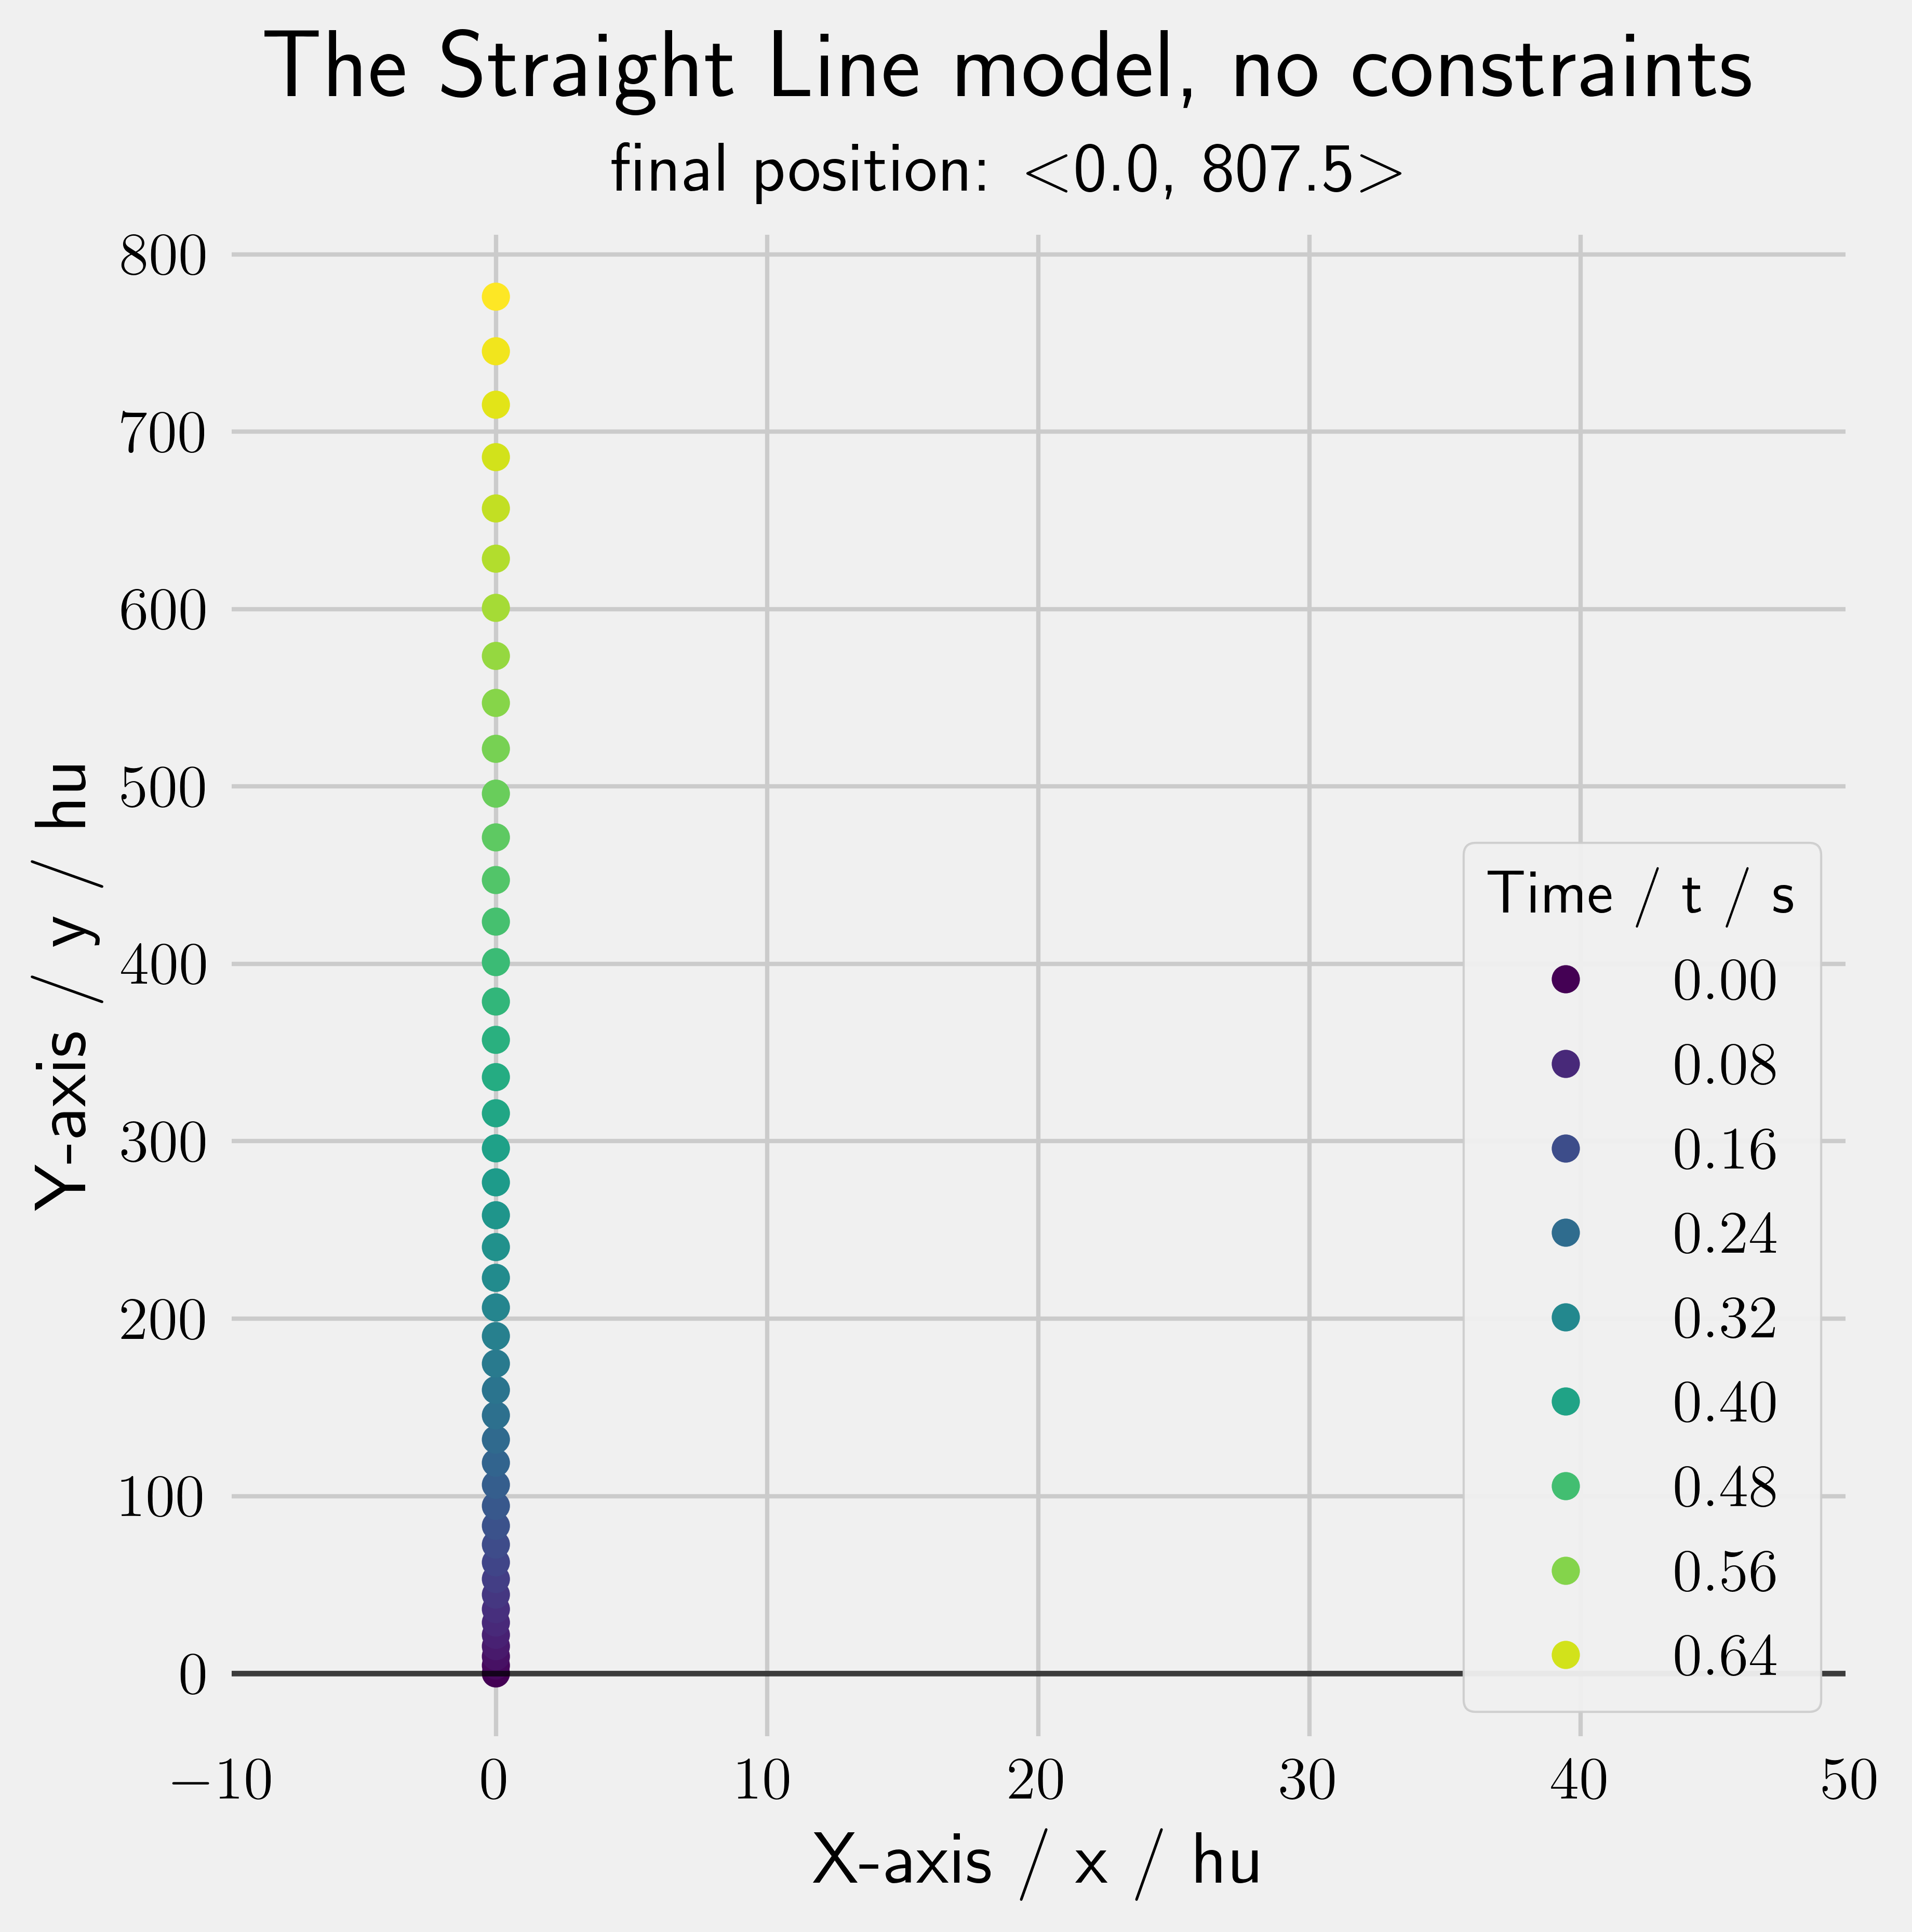
\includegraphics[width=0.45\textwidth,right]{assets/straight_nothing_1.png}
    \caption{}
    \label{fig:straight_nothing_1}
\end{wrapfigure}

I can comfortably say that this jumping distance would never be possible to achieve in game, for this model can be proven to be the most optimal jumping path if there are no speed limits (appendix, using EL equation). This number of around $900$ hammer units serves to be the upper-bound output of our optimization, and the lower-bound being its negative of around $-900$ (if you wish to accelerate directly backwards with negative initial velocity).

Additionally we can also utilize the equation derived in the last section (equations \ref{eq:jumping}).

Using the acceleration function, we can define $x(t)$ and $y(t)$ as:
\[
    x(t) = 0, \quad y(t) = 1.
\]

Their first and second order indefinite integrals can be obtained using calculus:
\begin{alignat*}{3}
    X(t) &= \int x(t) \, dx = 0, \quad
    &&\tfx(t) &&= \int X(t) \, dx = 0\\
    Y(t) &= \int y(t) \, dx = t, \quad
    &&\tfy(t) &&= \int Y(t) \, dx = \frac{1}{2} t^2,
\end{alignat*}
notice that the constants during integration are omitted as we've incorporated them into the derivation of the jumping motion equations as $c_1$, and $c_2$.

Therefore the $x$ position after $t_f$ seconds assuming no speed limit is:
\begin{align*}
    p_x &= p(t_f)_x = w\tfx(t_f) + t_f(v_{0x} - w\tfx'(0)) - w\tfx(0)\\
    &= w \times 0 + t_f(0 - w \times 0) - w \times 0\\
    &= 0,
\end{align*}
and the respective $y$ position is:
\begin{align*}
    p_y &= p(t_f)_y = w\tfy(t_f) + t_f(v_{0y} - w\tfy'(0)) - w\tfy(0)\\
    &= w \frac{1}{2} t_f^2 + t_f(v_{0y} - w v_{0y} \times 0) - w \times 0\\
    &= (12 \times 250) \frac{1}{2} (0.7)^2 + 0.7 \times 250\\
    &= 910.
\end{align*}

% TODO: change A to 10

The jumping motion differential equations resulted in a similar sized jumping distance of $910$ is comparison to the engine simulated $\approx934$. I believe that a $\frac{|910-934|}{934} \approx 2.57\%$ error is a very well approximation of this continuous method for future modeling.

\begin{wrapfigure}{r}{0.48\textwidth}
    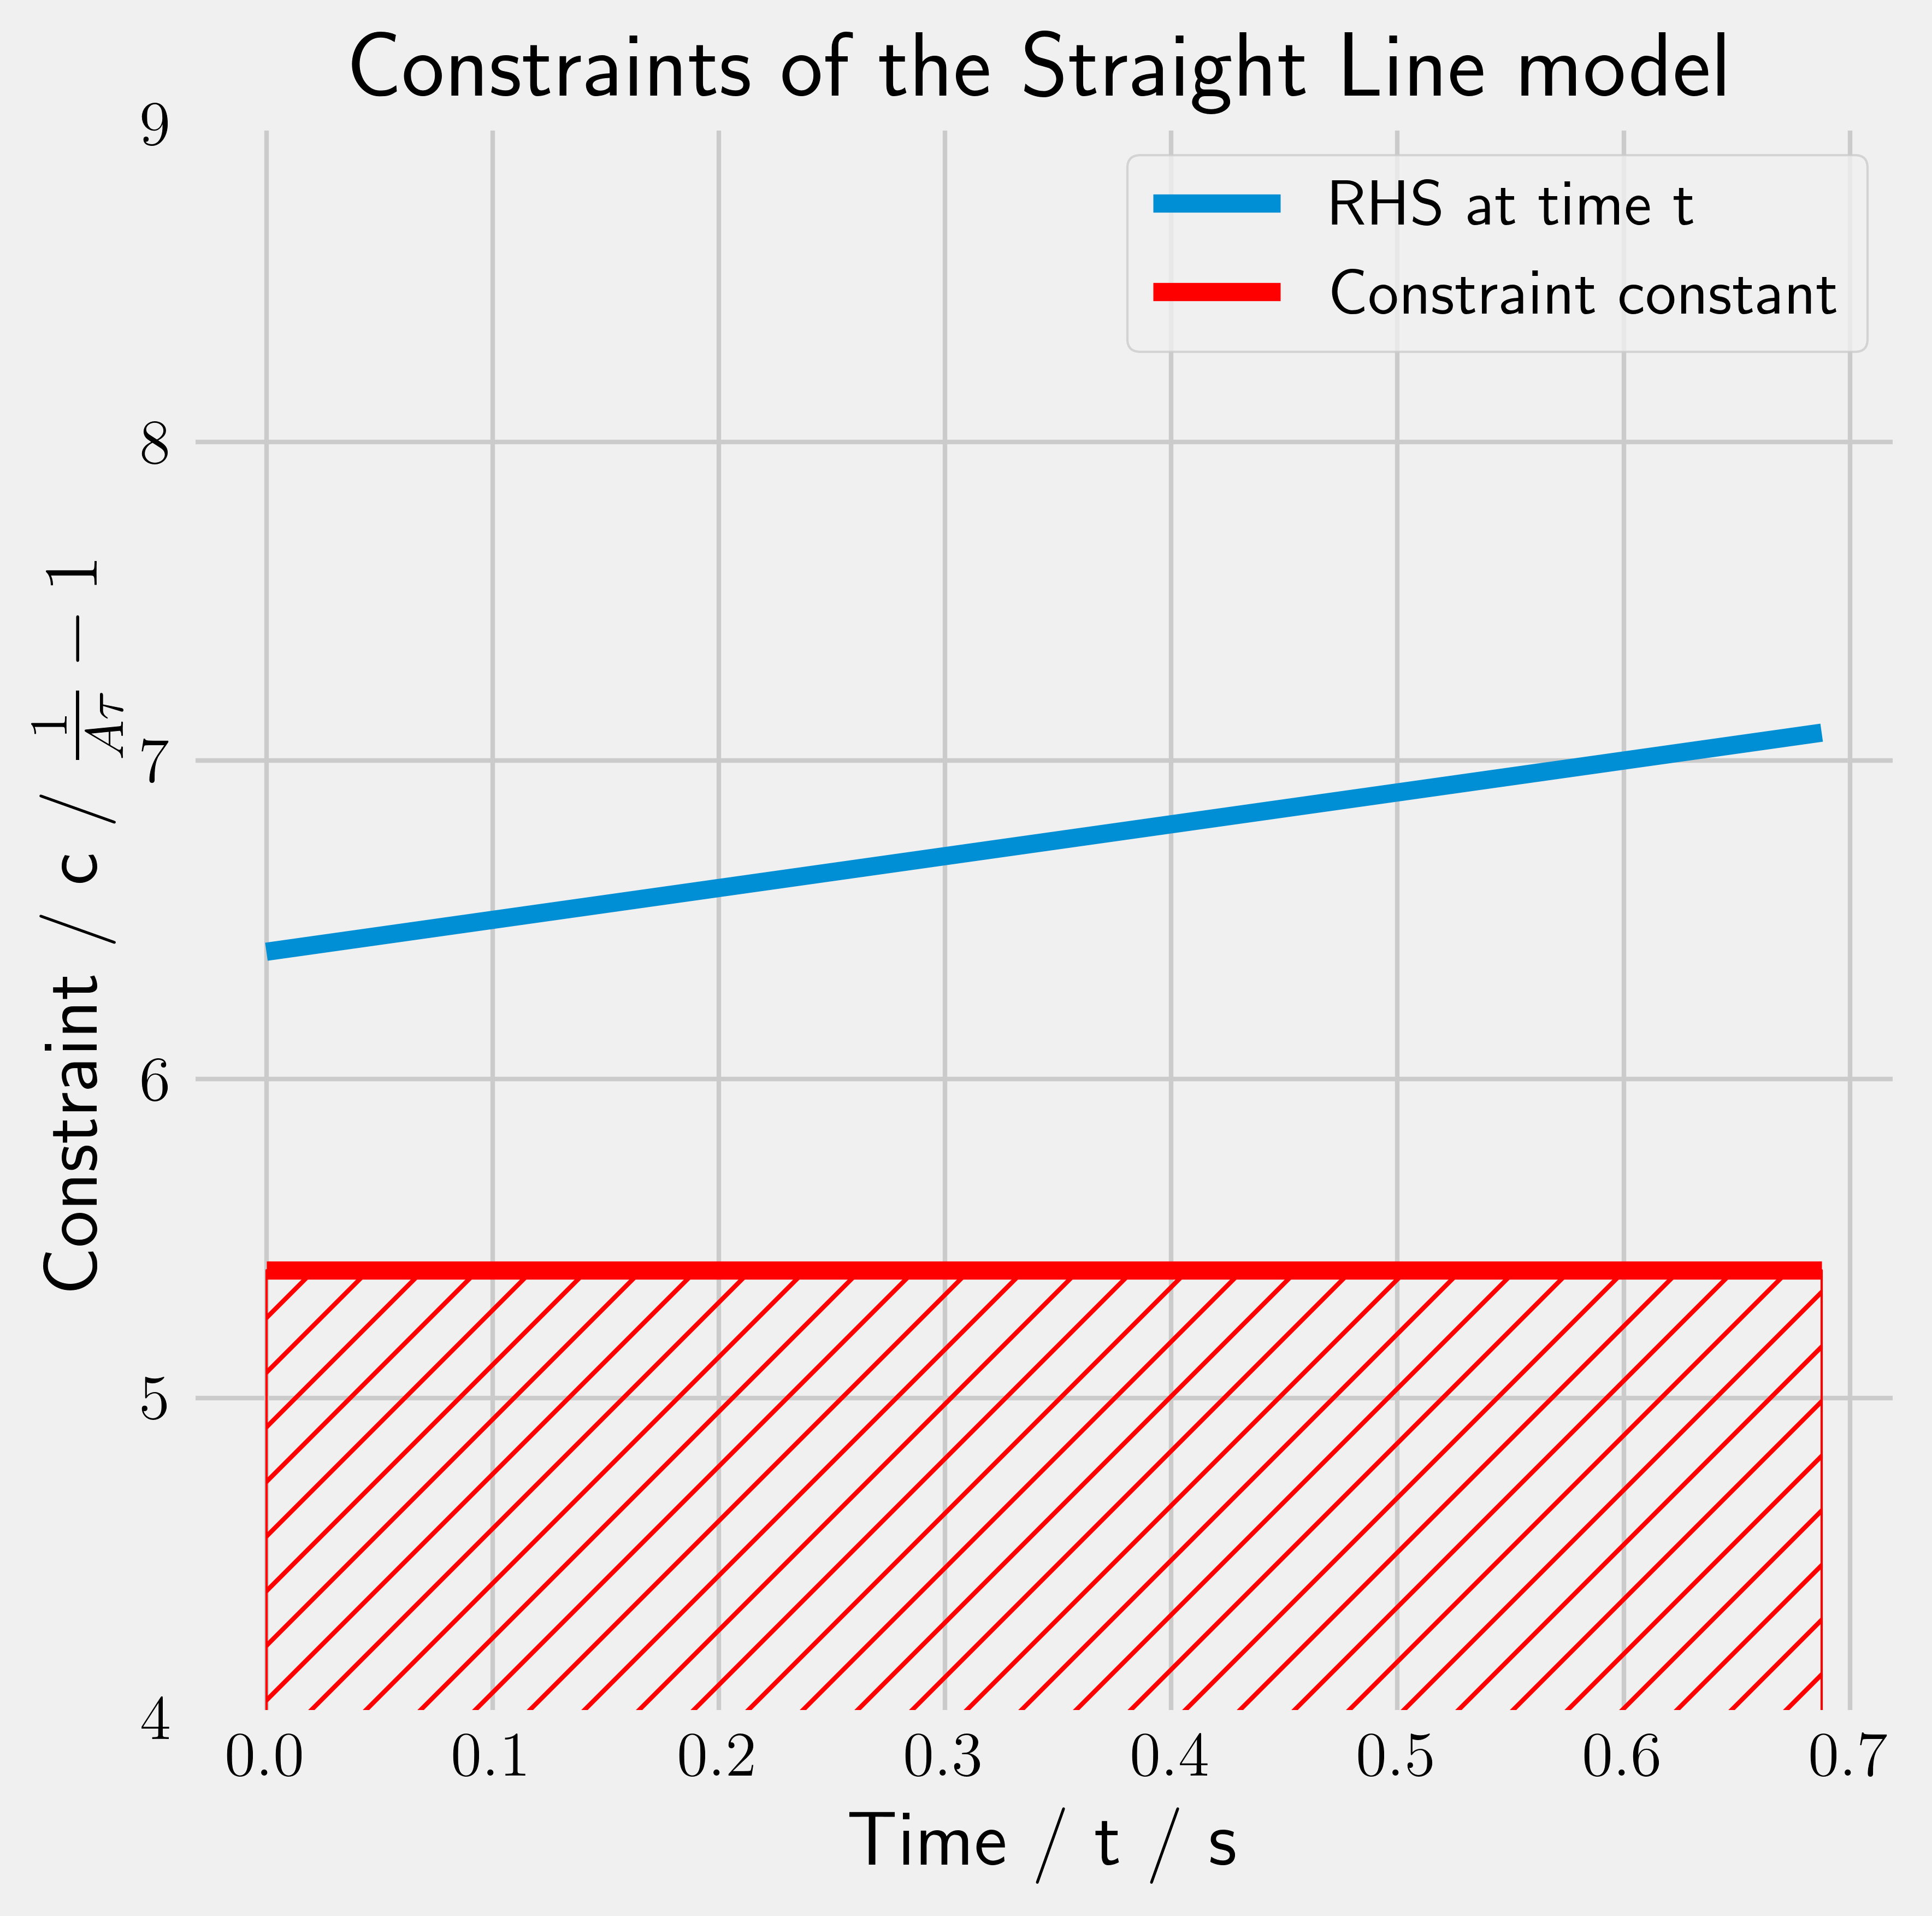
\includegraphics[width=0.45\textwidth,right]{assets/straight_constraint_inequality.png}
    \caption{}
    \label{fig:straight_constraint_inequality}
\end{wrapfigure}

But the game analyzed does have the constraint of a speed limit so players cannot accelerate infinitely, traveling across the map in two-to-three seconds. The graphing of the constraint (equation \ref{eq:constraint}) shows the problems (figure \ref{fig:straight_constraint_inequality}).



Blah blah blah one line is higher then the other,

% TODO: calculated the restricted line,

% TODO: conclude this: max 250 total words

% TODO Have around 1500 words

% 500 words each for each method

% 500 for conclusion

% Do the machine learning one

% Do the step by step one

% Do the euler-lagrange one

% Extension, find the optimal angle for each


\newpage
%

\section{Conclusion}
This essay explored the optimal jumping displacement of a player in ``Counter Strike, Source''. I first modeled the game with empirical data from the straight line model, deriving the mechanics behind jumping and researching the speed limit. In a case to avoid the speed limit, I've tested theories from both the skilled people and myself, and creating a modification to push the optimization further on the second discrete model. I believe that this exploration is useful towards the tool-assisted speedrun community, owning to the high amount of skill and precision needed for the advance models.



\nocite{*}
\newpage
\printbibliography

\end{document}
